\section{Introduction} \label{ch:intro}

%% P1: Multi-threading is critical and popular.
Multi-threading becomes increasing pervasive and critical because of two 
computing trends. First, due to the physical constraints on circuit speed, computers are having
more and more cores rather than faster and faster single-core. In order to 
harness the power of multi-core, developers write more and more multi-threaded programs . 
Second, the emerging cloud computing trend requires Internet services, ranging from 
web servers to storage engines, to process more and more requests at the same time, which also 
pushes developers to write more and more multi-threaded programs. These two trends continue and 
multit-threading becomes increaingly pervasive and critical.

%% P2: However, it is hard to get right.
Unfortunately, despite decades of effort from both academia and industry, 
multi-threaded programs are still notoriously difficult to get right. A key 
reason is: even running on the same input, the concurrently running threads of 
a program may interleave in \emph{too many} different ways, and we call these interleavings 
\v{schedules}. Considering all inputs, the number of possible schedules is even greater. 
In this traditional multit-threading manner, each input may run into too many 
thread interleavings, and each interleaving may process many different inputs.
This messy many-to-many mapping (Figure~\ref{fig:nondet}) makes existing techniques extremely
hard to test, analyze, and verify. As a result, a concurency bug hidden in one schedule can 
simply bypass existing reliability and security techniques in the testing lab and show up in the field, 
potentially causing program crashes, wrong outputs, security breaches, and so on.

%% P3: DMT: one possible approach. And its limitations.
In order to reduce the number possible schedules on each input, researchers 
have proposed a great idea called deterministic multithreading (or \dmt)~\cite{dthreads:sosp11,
dpj:oopsla09, dmp:asplos09, kendo:asplos09, coredet:asplos10} that 
always enforces the same schedule on the same input. By mapping each input to onely 
one schedule (Figure~\ref{fig:dmt}), \dmt greatly improved reliability for multithreaded programs on each input.
However, although \dmt is useful, it is not as useful as commonly perceived, 
because as we have shown in our previous research~\cite{cui:tern:osdi10},
a typical \dmt system can map slightly different inputs to 
very different schedules, artificially reducing programs' robustness on input 
perturbation, and the number of possible schedules on all inputs are still 
enorous, and the resultant programs are still very hard to test, analyze, verify, etc.

\begin{figure*}[t]
\begin{center}
\subfloat[{\em Traditional.}]{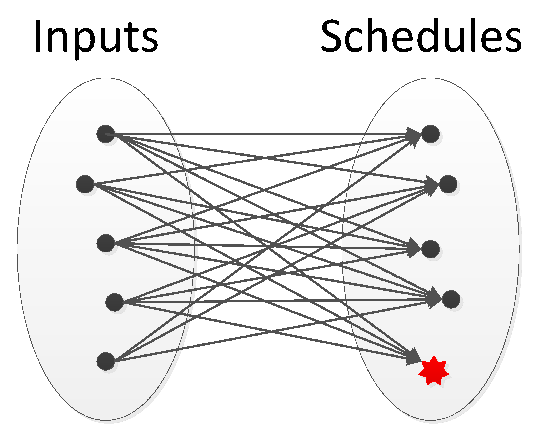
\includegraphics[width=.23\linewidth]{figures/nondet}\label{fig:nondet}}
\subfloat[{\em Deterministic.}]{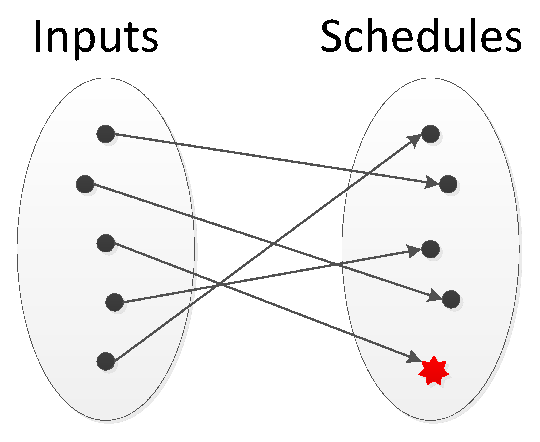
\includegraphics[width=.23\linewidth]{figures/dmt}\label{fig:dmt}}
\subfloat[{\em Stable (deterministic).}]{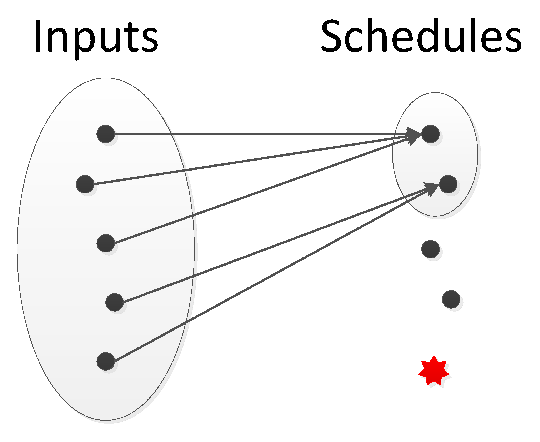
\includegraphics[width=.23\linewidth]{figures/smt}\label{fig:smt}}
\subfloat[{\em Stable (nondeterministic).}]{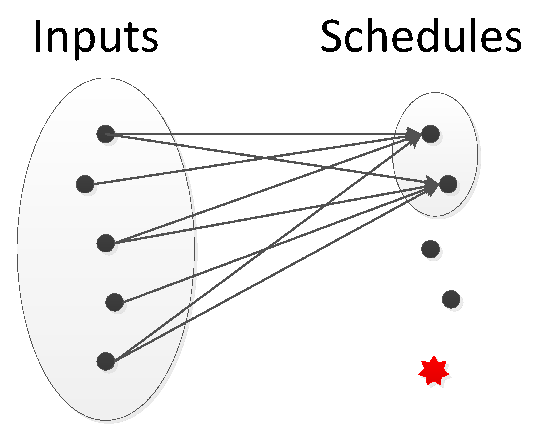
\includegraphics[width=.23\linewidth]{figures/smtn}\label{fig:smtn}}
\vspace{-.05in}
\caption{Different multithreading approaches. Red stars represent buggy
  schedules.  Traditional multithreading (\subref*{fig:nondet})
  is a conceptual many-to-many mapping where one input may execute under
  many schedules because of nondeterminism, and many inputs may execute
  under one schedule because a schedule fixes the order of the
  communication operations but allows the local computations to operate on
  any input data.  \dmt (\subref*{fig:dmt}) may
  map each input to an arbitrary schedule, reducing programs' robustness
  on input perturbations.  \smt (\subref*{fig:smt} and
  \subref*{fig:smtn}) reduces the total set of schedules for all inputs (
represented by the shrunk ellipses),
  increasing robustness and improving reliability.
  \smt and \dmt are orthogonal: a \smt system can be deterministic
  (\subref*{fig:smt}) or nondeterministic (\subref*{fig:smtn}).}
\vspace{-.2in}
\end{center}
\end{figure*}

%% P4: StableMT: our new approach and thesis.
We attacked this root cause by asking: are \emph{all} the enormously
many schedules necessary?  Our study reveals that \emph{many real-world
  programs can use a small set of schedules to efficiently process a wide
  range of inputs}~\cite{cui:tern:osdi10}.  Leveraging this insight, we
envision a new approach we call \emph{stable multithreading (\smt)}
that reuses each schedule on a wide range of inputs, mapping all inputs to a dramatically
reduced set of schedules. By vastly shrinking the haystack, it makes the
needles much easier to find.  By mapping many inputs to the same schedule (Figure~\ref{fig:smt}),
it stabilizes program behaviors against small input perturbations. 
\smt and \dmt are not mutually exclusive: a system can be both
deterministic and stable.

%% P5: StableMT's applications.
By greatly reducing the number of possible schedules for all inputs, \smt can benefit many reliability 
techniques and make it much easier to find the schedules that cause concurrency 
bugs. For example, my collaborators and I have quantitatively shown that \smt can 
increase the coverage of tools that systematically testing schedules for 
bugs~\cite{parrot:sosp13, dbug:spin11, modist:nsdi09}, and improve the precision 
of program analysis~\cite{wu:pldi12}, verification~\cite{wu:pldi12}, and 
debugging concurrency bugs~\cite{cui:tern:osdi10}. Some of our \smt techniques have 
also been used by other researchers to compute schedules for covering all 
inputs~cite{bergan:oopsla13}. We also plan to leverage \smt to enable transparent 
state-machine replication~\cite{paxos} for multi-threaded prograsms.

%% P6: intro to the systems we built: with each addressing different challenges.
Although the vision of stable multithreading is appealing, realizing it
faces numerous challenges.  Three main challenges are:

\begin{enumerate}

\item[$\bullet$] How can we compute the schedules to map inputs to?  The 
schedules
  must be feasible so executions reusing them do not get stuck.
  They should also be highly reusable.

\item[$\bullet$] How can we enforce schedules deterministically and
  efficiently?  ``Deterministically'' so executions that reuse a schedule
  cannot deviate even if there are data races, and ``efficiently'' so
  overhead does not offset reliability benefits.
  This challenge is also a decades-long challenge in the area of
  deterministic execution and replay.

\item[$\bullet$] How can we make \smt simple and deployable? To make sure 
  the schedules we checked are the schedules we run, \smt must be 
 deployed in the field as well as in the testing lab, then ``simplicity" and 
 ``deployability" are critical for adoption.

\end{enumerate}

Over the past four years, we have been tackling these challenges and
building \smt systems, which resulted in three \smt systems,
\tern~\cite{cui:tern:osdi10}, \peregrine~\cite{peregrine:sosp11}, and
 \peregrine~\cite{peregrine:sosp11}, with each system addressing each above challenge.
 Our solutions to these challenges will be described in the following sections.
 Our solutions are by no means the only
 ones; subsequent to \tern, others have also built a system that
 stabilizes schedules for general multithreaded programs~\cite{dthreads:sosp11}.

%% P7: Structures of this proposal.
The rest of this article is orgnized as follows. \S\ref{sec:tern} introduces \tern, 
\S\ref{sec:peregrine} introduces 
\peregrine, \S\ref{sec:parrot} introduces \parrot, \S\ref{sec:mc} introduces our 
application on improving schedule coverage for model checking,
\S\ref{sec:rep} introduces replication system \msmr, \S\ref{sec:related} introduces 
related work, and \S\ref{sec:plan} describes my research plan.

